\documentclass[paper=a4, fontsize=10pt]{scrartcl}

\usepackage{amsmath}
\usepackage[italian]{babel}
\usepackage{tabularx,ragged2e,booktabs,caption} % for table title
\setlength{\parskip}{0.5em} % for paragraph spacing
\DeclareOldFontCommand{\bf}{\normalfont\bfseries}{\mathbf} %declare \bf command in scrartcl

\pagenumbering{gobble} % remove the number of pages

\usepackage{graphicx} % per aggiungere figure/foto

\usepackage{sectsty} % Allows customizing section commands
\allsectionsfont{\normalfont\scshape} % Make all sections, the default font and small caps


%%
\usepackage[utf8]{inputenc}
\newcommand{\approxtext}[1]{\ensuremath{\stackrel{\text{#1}}{\approx}}}
%% now i can add a comment on top of “equal” and “approximate” symbols



\newcommand{\horrule}[1]{\rule{\linewidth}{#1}} % Create horizontal rule command with 1 argument of height

\title{	
\normalfont \normalsize 
\textsc{Universit\`a degli Studi di Trieste - Dipartimento di Ingegneria e Architettura} \\ [25pt] % Your university, school and/or department name(s)
\horrule{0.5pt} \\[0.4cm] % Thin top horizontal rule
\huge \textbf{Relazione progetto Reti Logiche\\ Weather Station}  \\ % The assignment title
\horrule{2pt} \\[0.5cm] % Thick bottom horizontal rule
}

\author{Andrea Gonzato} % Your name

\date{\normalsize Maggio 2019} % Today's date or a custom date

\setlength{\parindent}{0cm}

\begin{document}
\maketitle % Print the title

\pagebreak

\tableofcontents

\pagebreak

\section{Introduzione}
Questa è la relazione del progetto di Arduino svolto per il corso di reti logiche tenuto dal Professore Marsi dell'Università di Trieste.

\section{Scopo del progetto}
Lo scopo del progetto "Weather Station", da come suggerisce il nome è quello di realizzare una stazione meteorologica amatoriale. In aggiunta all'opportunità di poter visualizzare la temperatura e l'umidità attuale, sono state aggiunte funzionalità secondarie come la possibilità di poter leggere l'ora, data attuale e di poter utilizzare la stazione anche come fosse una sveglia. Ovviamente è previsto che data ora e sveglia possono essere regolate e la sveglia inoltre sia anche disattivabile.

\subsection{Descrizione per l'utilizzo}
Per controllare la stazione meteorologica ci sono tre pulsanti: \textit{SET}, \textbf{+}, \textbf{-}.
Il funzionamento ricorda molto l'utilizzo dei classici orologi da polso digitali. Dunque per poter scorrere lungo tutte le funzionalità si utilizzano i pulsanti \textbf{+} e \textbf{-}, mentre per impostare data, ora e sveglia si necessita di tener premuto per un secondo il pulsante \textit{SET}, dopodichè nella regolazione si usano gli analoghi pulsanti per aumentare e diminuire, mentre per passare a impostare il campo successivo oppure per attivare/disattivare la sveglia si necessita di premere una singola volta il pulsante \textit{SET}.


\subsection{Specifiche}
Come principali specifiche da rispettare, era necessario che l'orologio abbia una precisione che permetta di regolarlo mensilmente. Quindi ragionevolmente si richiedeva un errore inferiore di un secondo dopo 24 ore dalla sincronizzazione con un orologio affidabile.

Le altre specifiche sui dati meteo richiedono un errore inferiore a 1 grado Celsius per la temperatura e 2 punti percentuali per l'umidità.

\subsection{Risultato ottenuto}
In figura \ref{fig:progettoFoto} si può vedere la realizzazione del progetto completato.

Tutte le specifiche nella realizzazione finale del progetto sono state rispettate.

Ne suo complesso il sistema si può ritenere funzionante, stabile e facile nell'utilizzo.

\begin{figure}
  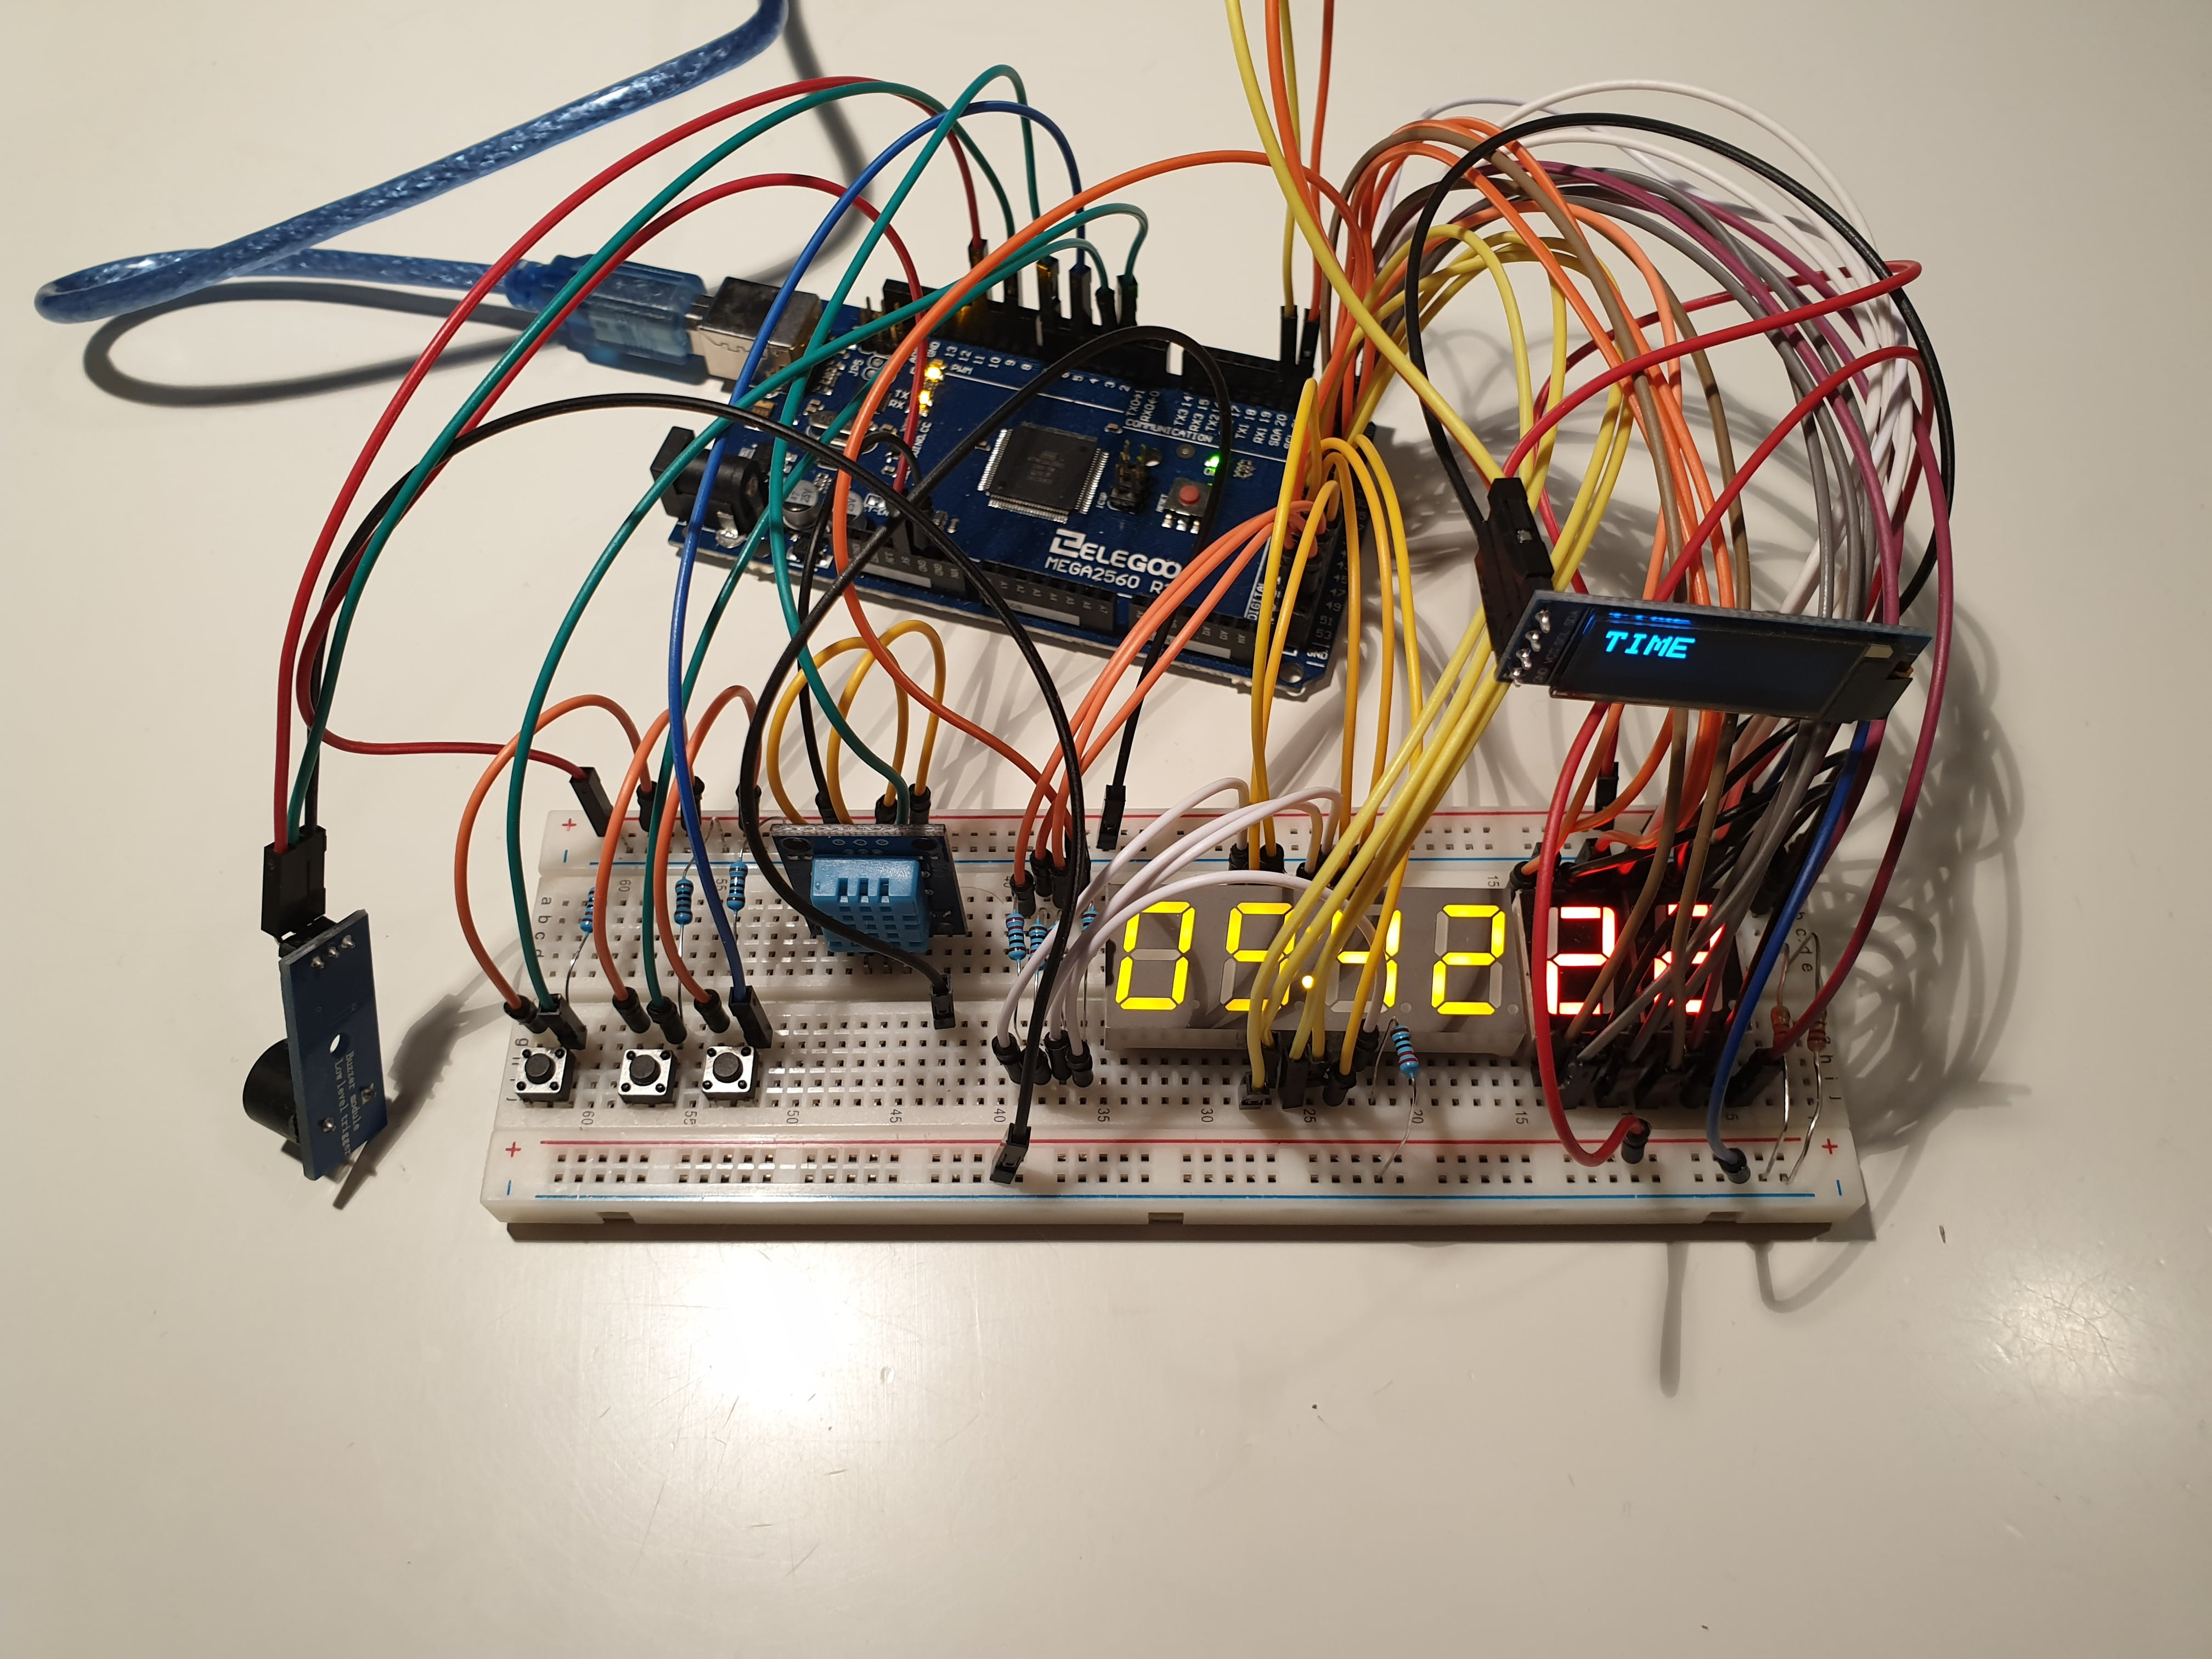
\includegraphics[scale=0.05]{projectPhoto.jpg}
  \caption{una immagine della realizzazione del progetto}
  \label{fig:progettoFoto}
\end{figure}
    

\section{Realizzazione}
Tutto il progetto è stato realizzato tra Marzo 2019 e Maggio 2019.\\

\subsection{Metodo usato}
Il primo periodo è stato utilizzato per recuperare il materiale necessario. Una volta reperiti i componenti sono stati eseguiti una serie di test per comprendere l'utilizzo e le capacità dei singoli componenti.

Nella seconda fase, momento in cui è iniziata la vera realizzazione del progetto, la metodologia adottata era ispirata al paradigma AGILE: Si aggiungevano funzionalità una alla volta passando ciclicamente da una fase di progettazione a sviluppo per poi passare ai test e verificare la correttezza delle implementazioni.

\begin{figure}
  
\includegraphics[scale=0.2]{AGILE.jpeg}
  \caption{paradigma AGILE}
  \label{fig:agile1}
\end{figure}
    
La figura \ref{fig:agile1}
illustra bene il paradigma adottato.


Nell'ultima fase del progetto, una volta implementata gran parte delle funzionalità, c'era la necessità di ristrutture il codice, creando una nuove versione strutturata ad oggetti, per poter avere un codice più leggibile ed uniforme.

\pagebreak

\subsection{Struttura della programmazione ad oggetti implementata}
Di seguito viene fornita una breve descrizione di come è stato strutturato ad oggetti il progetto.

Tutti gli oggetti vengono creati nel file \textit{Code/code.ino} e per ogni classe viene implementato un solo oggetto apparte per la classe \textit{Button} dove ne vengono creati tre. I metodi "principali" di ogni classe si chiamano \textit{update()} e in tali metodi i vari oggetti comunicano tra di loro i cambiamenti registrati durante il ciclo di eseguzione della funzione \textit{loop()}

Le classi implementate sono:

\begin{itemize}
\item MyTime: una classe che contiene tutte le variabili temporali e scandisce nel tempo l'evoluzione del sistema, questa classe serve per esempio per l'attivazione dell'allarme della sveglia.

\item Mode: una classe che gestisce e aggiorna il sistema informandolo su cosa bisogna visualizzare sui display a 7 segmenti: nella stazione meteo ci sono 5 dati fondamentali da far vedere all'utente che sono: tempo, data, temperatura, umidità, e l'orario a cui è impostata la sveglia. Ma osserva che per questioni progettuali sono uno alla volta di questi dati può essere visualizzato sui display.

\item Button: una classe che gestisce tutte le attività che iniziano alla pressione di un pulsante, per esempio aggiorna il sistema comunicando che durante un settaggio si è premuto un pulsante per far aumentare le ore dell'orologio. Questa classe è in continua comunicazione con MyTime e Mode.

\item controllSingleDigitDisplay: una classe che si occupa di visualizzare i dati richiesti sui 2 display a 7 segmenti 1 digit.
\end{itemize}


\subsection{Componenti utilizzati}
Dopo aver definito le specifiche, durante la prima fase è stato necessario reperire tutto il materiale necessario.\\
Questa è una lista completa del materiale utilizzato
\begin{itemize}
\item Arduino Mega 2560
\item breadboard (63x10)
\item sensore digitale DHT11 per rilevare temperatura e umidità
\item schermo OLED (risoluzione: 128*32)
\item display 7 segmenti (4 digits, catodo comune)
\item 2 display 7 segmenti (1 digit, catodo comune)
\item cicalino (buzzer passivo)
\item 3 bottoni
\item 7 resistenze da 220 Ohm
\item 3 resistenze da 1k Ohm
\item 50/55 cavi elettrici M/M
\item 8 cavi elettrici M/F
\end{itemize}

Si osservi che per la realizzazione di questo progetto non è sufficiente un Arduino Uno perché, da come si vede in Figura \ref{fig:schema1}, sono necessarie 34 connessioni digitali.
\subsection{Schema}
In fono alla relazione si può osservare la figura \ref{fig:schema1} che indica lo schema utilizzato per il progetto.

Nota che nello schema non sono presenti le connessioni, del cicalino e dello schermo OLED. Ma queste sono particolarmente semplici e intuitive. Se si vuole usare il codice del progetto, i pin del cicalino I/O e VCC vanno connessi rispettivamente a i pin Arduino 9 e 11.


\subsection{Strumenti usati}
I principali strumenti che sono stati utilizzati sono: l'ambiente Arduino e Fritzing come software per disegnare gli schemi elettronici.\\
Nel codice del progetto sono presenti come librerie esterne:
\begin{itemize}
\item \textit{SevSeg}
\item \textit{DHT}
\item \textit{Adafruit Sensor}
\item \textit{Adafruit GFX}
\item \textit{Adafruit SSD1306}
\end{itemize}

\textit{SevSeg} è stata utile per "scrivere" sul display a 7 segmenti 4 digits; mentre \textit{DHT} e \textit{Adafruit Sensor} sono servite per leggere i dati dal sensore che rilevava la temperatura e l'umidità; infine  le ultime due librerie hanno permesso di utilizzare lo schermo OLED. 


\subsection{Scelte progettuali e difficoltà}
Una scelta progettuale effettuata, consisteva nel scegliere come far scandire il tempo al sistema.
La prima opzione consisteva nell'acquisire un modulo RTC appositamente designato per queste attività; ma la scelta progettuale invece attuata è stata di far scandire il tempo direttamente ad Arduino, creando una variabile \textit{long unsigned} che incrementa al passare di ogni millisecondo. Scegliendo questa realizzazione si è riusciti a risparmiare un modulo ma ad un costo: infatti la variabile teoricamente dopo 4,294,967,295 millisecondi, cioè circa in 49 giorni arriva in overflow e questo potrebbe portare in crash il sistema (questo avvenimento non è ancora stato testato). Per questo motivo sopracitato si raccomanda di resettare la stazione prima dello scadere del quarantottesimo giorno.

La difficoltà più grande incontrata è stata sicuramente, quella di gestire e sincronizzare i display a 7 segmenti. Nel progetto originale, l'idea era quella di realizzare il sistema di visualizzazione dati utilizzando due display a 7 segmenti con 4 digits, quindi poter disporre di un totale di 8 digits. Il problema di questa realizzazione era che la libreria \textit{SevSeg} utilizzata non supportava l'opportunità di comandare più display contemporaneamente. Per tale motivo la realizzazione finale del progetto è avvenuta con l'implementazione di un display 4 digits controllato dalla libreria, affiancato da due display sigle digit controllati senza libreria ma con comandi standard \textit{digitalWrite()} di Arduino. Questo compromesso ha reso l'aggiornamento dei display non uniforme e non ottimizzato, infatti ad ogni eseguzione dell'\textit{loop()} ciclicamente un solo digit del display composto da quattro si aggiorna, mentre entrambi i display single digit si aggiornano. In futuro, si dovrebbe migliorare questa non uniformità nell'illuminazione dei display. Ma attualmente non si ritiene sia fondamentale.

Come protocollo di comunicazione tra il display OLED e Arduino si è deciso di utilizzare il protocollo $I^{2}C$ considerando il fatto che l'Arduino Mega 2560 possiede due pin addetti per tale scopo.

L'utilizzo della libreria \textit{SevSeg} ha portato come compromesso che all'interno del \textit{loop()} non possa essere inserito alcun ritardo di qualunque tipo. In caso questi avvenissero, il display a 7 segmenti 4 digits inizia a sfarfallare. A causa di questa problematica il sensore di umidità e temperatura rileva i dati non in maniera continuata, ma esclusivamente ogni 20 secondi. Questo perché altrimenti si verificherebbero dei ritardi nell'\textit{loop()}. Infatti se si osserva bene il display, ogni 20 secondi c'è un piccolo sfarfallamento, ma non è particolarmente fastidioso.




\section{Sviluppi futuri}
I prossimi sviluppi per questo progetto riguarderanno aspetti secondari.
Di seguito vengono elencate alcune possibili futuri sviluppi per il progetto:
\begin{itemize}
\item introduzione di nuove melodie più piacevoli per la sveglia.

\item introduzione di una nuova funzionalità che permetta l'uso della stazione anche come cronometro.

\item introduzione di una nuova funzionalità che permetta l'uso della stazione anche come timer.

\item implementazione di un sensore che rilevi la pressione (barometro) e di una funzionalità che permetta di vedere il suo stato attuale.

\item introduzione di effetti sonori, durante le attività di settaggio degli strumenti.

\item implementazione di un sistema di memorizzazione che scriva i dati meteorologici (temperatura, umidità e pressione) in una scheda sd. Permettendo di creare degli storici/report sui dati rilevati.

\end{itemize}


\section{Rilascio materiale}
Tutto il materiale di questo progetto è rilasciato il licenza open source ed è reperibile al seguente sito:
\textit{https://github.com/AndreaGonzato/WeatherStation}

In questa pagina è possibile trovare anche la vecchia versione del codice non strutturato ad oggetti. Tale versione, chiamata \textit{"Code No OOP"}, non supporta le ultime funzionalità come ad esempio la sveglia; ma può rilevarsi utile per chi intende contribuire a questo progetto ma non è molto famigliare con la programmazione ad oggetti.


\section{Conclusioni}
Sicuramente il progetto non è ne perfetto ne completo, ma nel suo complesso si può definire un prototipo funzionante.

\section{Sitografia}

Le librerie utilizzate sono reperibili ai seguenti siti:
\begin{itemize}
\item https://github.com/DeanIsMe/SevSeg
\item https://github.com/adafruit/Adafruit-GFX-Library
\item https://github.com/adafruit/Adafruit\_SSD1306
\item https://github.com/adafruit/DHT-sensor-library
\item https://github.com/adafruit/Adafruit\_Sensor
\end{itemize}

Altri siti dove sono state lette guide e tutorial
 sono:


\section{Dichiarazione finale}
Tutto il lavoro è stato svolto da me in completa autonomia.

\begin{figure}
  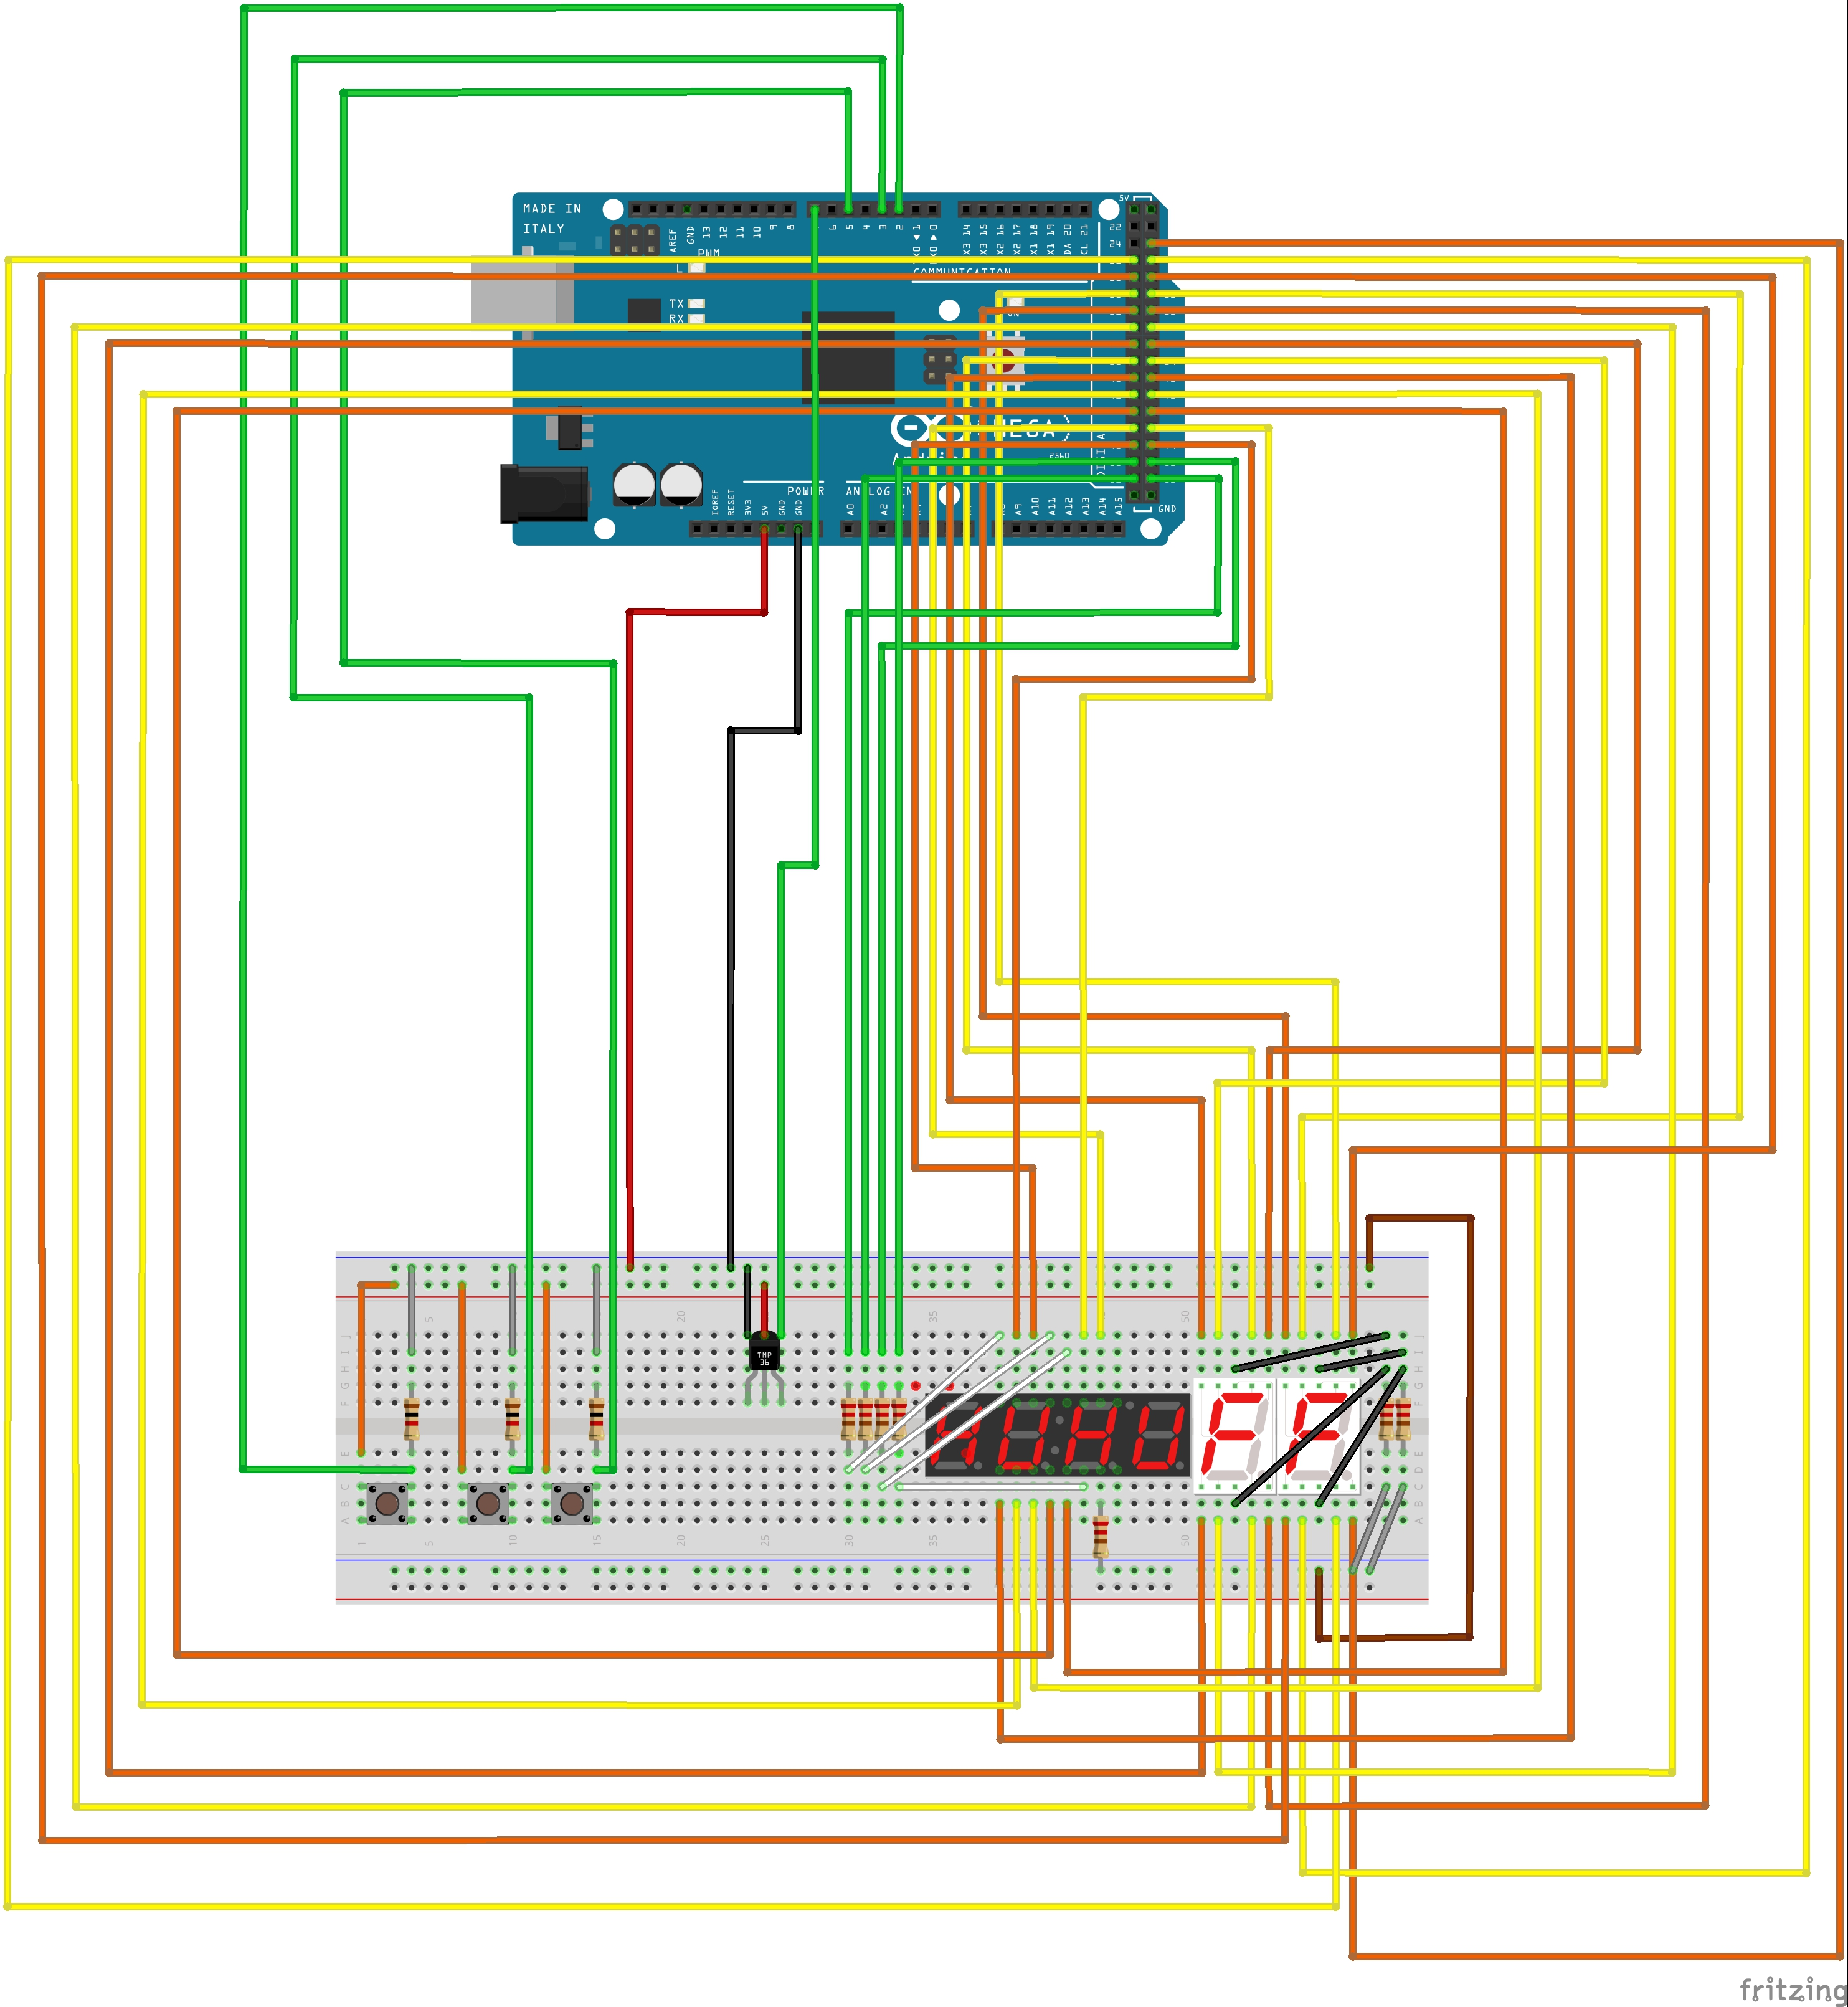
\includegraphics[width=\linewidth]{MySchema.jpg}
  \caption{Schema del circuito}
  \label{fig:schema1}
\end{figure}

\end{document}